\section{Einleitung}
\label{Einleitung}

\subsection{Motivation}
\label{Motivation}
	Energie zu sparen ist seit Langem ein Ziel der Umweltpolitik, dennoch steigt der Energieverbrauch in Industriel"andern kontinuierlich und es werden nach wie vor Wege gesucht, diesen zu senken. 
	In den USA verursachen private Haushalte 40\% des CO2-Aussto{\ss}es \cite{vandenbergh2008individual} und stehen deshalb im Fokus vieler Programme zum Energiesparen. \\
	Je nach Studie besteht f"ur die Haushalte ein Einsparungspotential von bis zu 20\% \cite{armel2013disaggregation} für dessen Energieverbrauch, Fischer \cite{fischer2008feedback} untersucht mehrere dieser Studien und beschreibt ein durchschnittliches Einsparungspotential von 5-12\%. 
	Um dieses Einsparungspotential auszunutzen, muss der Nutzer regelm"a{\ss}ig und m"oglichst genau "uber seinen Verbrauch aufgekl"art werden. 	%TODO Graphik Armel
	\begin{figure}[ht]
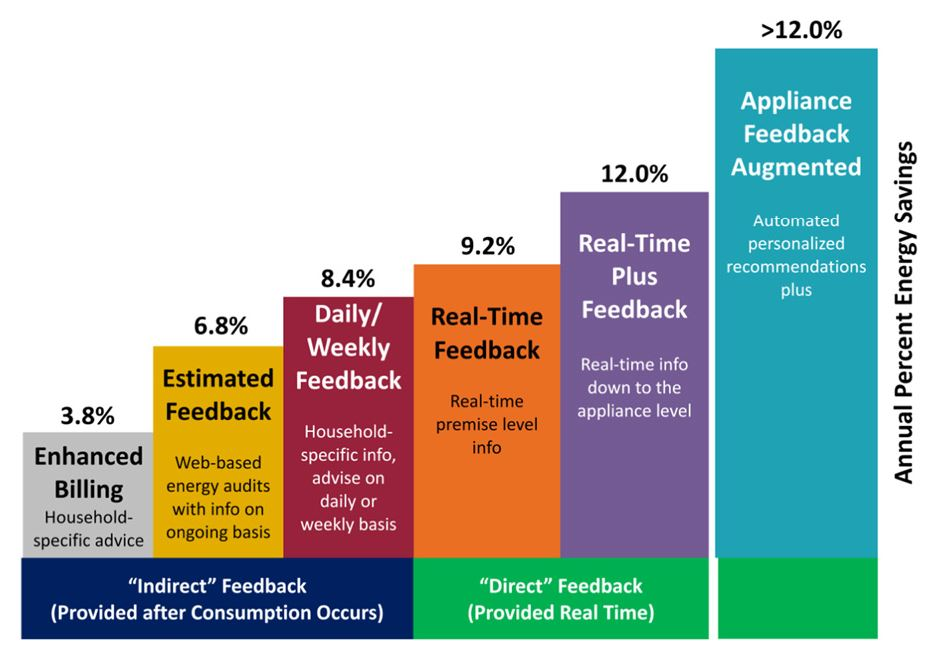
\includegraphics[height=0.7\textwidth]{1_Grafiken/fig1armel.jpg}
	\caption[Einsparungpotentiale nach Ma{\ss}nahme]{Grafik zu Einsparpotetialen je nach getroffener Aufkl"arungsma{\ss}nahme aus \cite{armel2013disaggregation}}
\label{potentiale}
\end{figure}

	Er kann sich oft nicht mit seinem Verbrauch identifizieren, weil dieser intransparent und durch die langen Rechnungsintervalle nicht pr"asent ist. \\
	Damit der Nutzer anf"angt sich selbst zu kontrollieren, muss er begreifen, dass sich sein Verhalten auf seinen Verbrauch auswirkt und er ihn auch durch die gezielte Ver"anderungen seines Handelns senken kann \cite{fischer2008feedback}.\\
	Non-intrusive load monitoring (NILM) bietet nun die Chance dem Nutzer eine regelm"a{\ss}ige, detaillierte R"uckmeldung zu seinem Energiekonsum zu geben, Kolter und Matthew \cite{kolter2011redd} beschreibt NILM als die Aufgabe aus einem, f"ur den gesamten Haushalt messenden Stromz"ahler, R"uckschl"usse "uber die elektrische Last einzelner Ger"ate zu ziehen.
	Ein solches System wird dem Konsumenten helfen, verschwenderische Verhaltensweisen und Ger"ate zu identifizieren ohne den Haushalt mit vielen digitalen Z"ahlern f"ur die individuellen Ger"ate ausr"usten zu m"ussen, wie es derzeit z.B. mit sogenannten \textit{Energiekostenmessger"aten} auf Steckerbasis praktiziert wird.

\subsection{Fragestellung}
\label{Fragestellung}
 	Viele Systeme zur Disagregation oder zu verschiedenen Vorhersage-Aufgaben benutzen Ans"atze des Maschinellen Lernens. Sie ben"otigen annotierte (gelabelte) Trainingsdaten, um robuste Modelle zu erzeugen. Annotieren bedeutet in diesem Zusammenhang, die Daten mit Metadaten wie etwa dem Ger"atezustand zu versehen. Mehr Trainingsdaten f"uhren in der Regel zu besseren Modellen, die Annotation ist allerdings sehr aufw"andig, weil sie manuell erfolgen muss. Der Ansatzpunkt dieser Arbeit ist, das Problem der Disagregation auf ein Ger"at zu reduzieren und so zu vereinfachen. Nun kann man ein robustes Modell mit nur wenigen Trainingsdaten erstellen und mit diesem dann eine gro{\ss}e Menge an Daten schnell annotieren. Diese gelabelten Daten sollen dann wiederum als Trainingsdaten f"ur schwierigere Aufgaben verwendet werden. 
	Aufgabe dieser Bachelorarbeit ist es ein System zu entwickeln, welches in der Lage ist die Zust"ande von ausgew"ahlten Ger"aten in einem disaggregierten Lastgang zu klassifizieren und so eine Segmentierung f"ur diese Ger"ate zu erstellen. Dies beinhaltet sowohl die n"otige Vorverarbeitung der Daten sowie eventuelle nachtr"agliche Formatierungen. Die eigentliche Klassifikation soll mit K"unstlichen Neuronalen Netzen (KNN) stattfinden, dabei sollte eine m"oglichst hohe Akkurarit"at erreicht werden, da Systeme, die mit den resultierenden Daten trainiert werden keine M"oglichkeit haben Fehler, die bereits in den Trainingsdaten sind, zu korrigieren. 

\subsection{Weiterer Aufbau}
\label{Weiterer Aufbau}
	Im folgenden Kapitel 2 werden die verwendeten, disaggregierten Energiedatens"atze beschrieben. Insbesondere werden die gemessenen Werte und die daraus berechenbaren Werte untersucht. 
	Kapitel 3 gibt zun"achst einen "Uberblick "uber die aktuelle Forschung im Bereich Vorverarbeitung der Daten und Feature-Auswahl, anschlie{\ss}end werden die f"ur diese Arbeit verwendeten Vorverarbeitungsschritte und Features erl"autert.
	In Kapitel 4 soll schlie{\ss}lich die eigentliche Klassifizierung beschrieben werden, hier werden insbesondere das verwendete Netz und die Trainingsmethoden besprochen. Auch hier wird es einen kurzen "Uberblick "uber die aktuelle Forschung geben.
	In Kapitel 5 findet die Klassifikation statt, hier werden verschiedene Klassifizierungsaufgaben ausgef"uhrt und ausgewertet. 
	Am Schluss steht das Fazit, in dem die Ergebnisse zusammengefasst und mit urspr"ungliche Fragestellung verglichen werden. 